
\section{\label{sec:tutorial:shearwave:tri3}2D Bar Discretized with Triangles}

PyLith features discussed in this tutorial:
\begin{itemize}
\item Dynamic solution
\item CUBIT format
\item Absorbing dampers boundary conditions
\item Kinematic fault interface conditions
\item Plane strain linearly elastic material
\item VTK output
\item Linear triangular cells
\item SimpleDB spatial database
\item ZeroDispDB spatial database
\end{itemize}
All of the files necessary to run the examples are contained in the
directory \texttt{examples/bar\_shearwave/tri3.}


\subsection{Mesh Generation}

The mesh is a simple rectangle 8 km by 400 m (Figure \ref{fig:shearwave:tet4:mesh}).
This mesh could be generated via a simple script, but it is even easier
to generate this mesh using CUBIT. We provide documented journal files
in \texttt{examples/bar\_shearwave/tri3.} We first create the geometry,
mesh the domain using triangular cells, and then create blocks and
nodesets to associate the cells and vertices with materials and boundary
conditions. See Section \ref{sec:Tutorial-3d-hex8} for more information
on using CUBIT to generate meshes.

\noindent \begin{center}
\begin{figure}
\begin{centering}
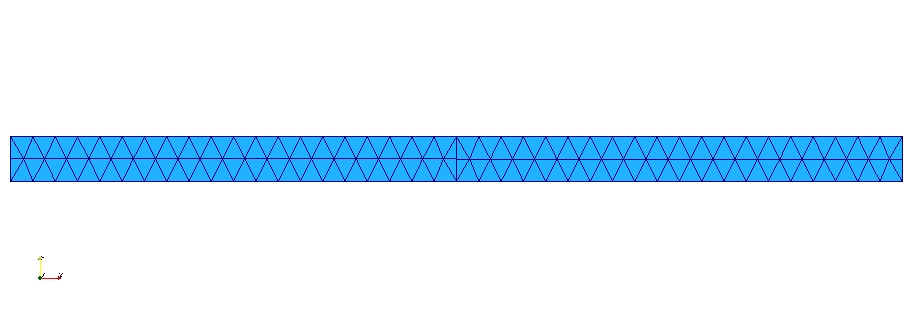
\includegraphics[scale=0.5]{tutorials/shearwave/figs/tri3mesh}
\par\end{centering}

\caption{Mesh composed of triangular cells generated by CUBIT used for the
example problem.\label{fig:shearwave:tri3:mesh}}
\end{figure}

\par\end{center}


\subsection{Simulation Parameters}

All of the parameters are set in the \texttt{pylithapp.cfg} file.
The structure of the file follows the same pattern as in all of the
other examples. We set the parameters for the journal information
followed by the mesh reader, problem, materials, boundary conditions,
fault, and output. We change the time-stepping formulation from the
default value of implicit time stepping to explicit time stepping
with a lumped Jacobian matrix by setting the formulation object via
\begin{lyxcode}
formulation~=~pylith.problems.Explicit
\end{lyxcode}
Using the Explicit object automatically triggers lumping of the Jacobian
cell matrices and assembly into a vector rather than a sparse matrix.
Lumping the Jacobian decouples the equations, so we can use a very
simple direct solver. Use of this simple solver is also triggered
by the selection of any of the Explicit formulation objects. 

For dynamic problems we use the NondimElasticDynamic object to nondimensionalize
the equations. This object provides scales associated with wave propagation
for nondimensionalization, including the minimum wave period, the
shear wave speed, and mass density. In this example we use the default
values of a minimum wave period of 1.0 s, a shear wave speed of 3
km/s, and a mass density of 3000 kg/m$^{3}$. We simulate 12.0 s of
motion with a time step of 1/30 s. This time step must follow the
Courant\textendash{}Friedrichs\textendash{}Lewy condition; that is,
the time step must be smaller than the time it takes the P wave to
propagate across the shortest edge of a cell. 

The boundary conditions include the absorbing dampers at the ends
of the bar and a Dirichlet boundary condition to prevent longitudinal
motion. Because we cannot overlap the Dirichlet BC with the fault,
we use the nodeset associated with all vertices except the fault.
For the output over the entire domain, we request both displacement
and velocity fields:
\begin{lyxcode}
{[}pylithapp.timedependent.output{]}

vertex\_data\_fields~=~{[}displacement,velocity{]}
\end{lyxcode}
To run the problem, simply run PyLith without any command line arguments:
\begin{lyxcode}
pylith
\end{lyxcode}
The VTK files will be written to the \texttt{output} directory. The
output includes the displacement and velocity fields over the entire
domain at every 3rd time step (0.10 s), the slip and change in traction
vectors on the fault surface in along-strike and normal directions
at every 3rd time step (0.10 s), and the strain and stress tensors
for each cell at every 30th time step (1.0 s). If the problem ran
correctly, you should be able to generate a figure such as Figure
\ref{fig:shearwave:tri3:deform}, which was generated using ParaView.

\noindent \begin{center}
\begin{figure}
\begin{centering}
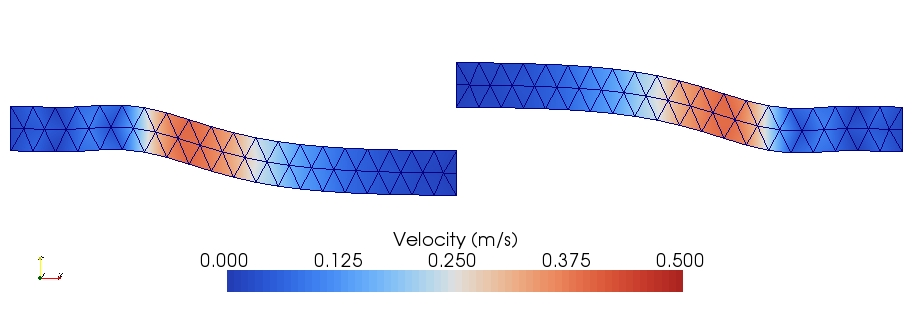
\includegraphics[scale=0.5]{tutorials/shearwave/figs/tri3deform30}
\par\end{centering}

\caption{Displacement field in the bar at 3.0 s. Deformation has been exaggerated
by a factor of 800.\label{fig:shearwave:tri3:deform}}
\end{figure}

\par\end{center}
